\documentclass[10pt]{article}

% required packages
\usepackage{graphicx}
\usepackage[hidelinks]{hyperref}
\usepackage{fancyhdr}

% margins
\setlength{\headwidth}{6.40in}
\pagestyle{fancy}
\addtolength{\textwidth}{1in}
\addtolength{\textheight}{1in}
\addtolength{\evensidemargin}{0.5in}
\addtolength{\oddsidemargin}{-0.5in}
\addtolength{\topmargin}{-0.5in}


% page headers
\fancyhead{} 
\fancyhead[LO,LE]{CSE 250B}
\fancyhead[RO,RE]{Project 1}



\title{Logistic Regression with L$_2$ Regularization}

\author{Adrian Guthals, David Larson, Jason Yao \\
CSE 250B: Project \#1 \\
University of California, San Diego \\
}


\begin{document}

\maketitle


\begin{abstract}
Logistic Regression with L$_2$ Regularization is analyzed as a classification learning method for data sets with real-valued features and binary labels. Stochastic Gradient Descent (SGD) and Limited-memory BFGS (L-BFGS) are used to find the regression parameters such that the Log Conditional Likelihood is maximized. The methods are applied to two common data sets: USPS-N (images of hand-written digits) and Web (statistics on HTML web pages). For the USPS-N data set, SGD had a (lower/equal/higher) test error than L-BFGS (xxx vs xxx) while for the Web data set, blah. These results indicate that blah blah blah about the two gradient methods as well as blah about logistic regression.
\end{abstract}



%-----------------------------------------------------------------------------
% INTRODUCTION
%-----------------------------------------------------------------------------
\section{Introduction}
\label{sec:intro}

Machine Learning (ML) is a sub-discipline of Artificial Intelligence (AI) that focuses on the development and analysis of methods that produce models from data. An often referenced example application of ML is email spam filtering, but there is a wide variety of real-world problems where ML has been successful used, from object detection using a Microsoft Kinect sensor \cite{Kinect} to forecasting of power output from a photovoltaic solar farm \cite{solar}.

ML algorithms are plentiful in number, but some are more suitable than others depending on the type of problem. Logistic regression is a ML algorithm well-suited to problems involving a set of real-valued inputs and a binary (Bernoulli) output. A real-world example of such a problem is whether a baseball player will hit a home run based on a collection of statistics (e.g. batting average, height, weight). The statistics are the real-valued inputs, whether he hits a home run is the binary output (1=yes, 0=no), and the probability of whether a player hits a home run is the determined using logistic regression. 

In this paper we analyze logistic regression's capability for classification learning using a previously study as a baseline \cite{t-logistic}. Aside from recreating the previous study's results, we also extend their work to comparing two gradient-based optimization methods for use in conjuction with the logistic regression: Stochastic Gradient Descent (SGD) and Limited-memory Broyden-Fletcher-Goldfarb-Shannon (L-BFGS).



%-----------------------------------------------------------------------------
% DESIGN OF ALGORITHMS
%-----------------------------------------------------------------------------
\section{Design and Analysis of Algorithms}
\label{sec:algorithms}

\subsection{Logistic Regression}
Given a set of real-valued features $x$ with binary labels $y$ (a training set), we can define logistic regression model as: 
\begin{equation}
    p_i = p( y_i | x_i ; \beta )  = \frac{1}{1 + \textrm{exp}-[\sum_{j=0}^d \beta_j x_ij]}
\end{equation}
where $d$ is the dimensionality of a training example, and $\beta_j$ are parameters of the regression. To learn the logistic regression, we need deteremine $\vec\beta$ such that the Log Conditional Likelihood (LCL) is maximized. In more formal notation:
\begin{equation}
   \widehat{B} = \textrm{argmax}_{\beta} \textrm{LCL}
\end{equation}
where LCL is defined as:
\begin{equation}
    \textrm{LCL} = \sum_{i:y_i=1} log (p_i) + \sum_{i:y_i=0} log (1-p_i)
\end{equation}
and is maximized when its derivative with respect to each parameter $\beta_j$ is zero. For a single example the partial derivative of the LCL is:
\begin{equation}
    \frac{\partial}{\partial \beta_j} log L(\beta ; x, y) = (y - p) x_j
\end{equation}


\subsection{L$_2$ Regularization}
In order to prevent overfitting of machine learning, a penalty was imposed to regulate the values of the parameters. A regularization constant $\mu$ was introduced into the LCL objective function:

\begin{equation}
    \hat{B} = \textrm{argmax}_{\beta} LCL - \mu||\beta||_2^2
\end{equation}
where $||\beta||_2^2$ is the $L_2$ norm of the parameter vector. With this revision the derivative of the LCL becomes:

\begin{equation}
    \frac{\partial}{\partial \beta_j} [ log p( y | x ; \beta) -\mu \sum_{j=0}^d \beta_j^2 ] = (y - p) x_j - 2 \mu \beta_j
\end{equation}


\subsection{Gradient-Based Optimization}
To efficiently maximize LCL, two gradient-based optimization methods are used: SGD and L-BFGS. The SGD was coded from scratched in Matlab while we used the popular minFunc toolbox \cite{minFunc} for the L-BFGS. For each of these algorithms, the input training data is formatted as a set of $n$ examples ($x_1, \ldots , x_n$) where each $x_i$ is a real-valued vector of $d$ features. Each $x_i$ is correlated to a binary (Bernoulli) outcome $y_i$ by a global parameter vector $\beta$ of length $d+1$. 


\subsubsection{SGD} 
Our SGD implementation first randomized the order of input examples to avoid repeated computation of random numbers and partitioned the input data into $x_1 \ldots x_k$ \emph{training} examples and $x_{k+1} \ldots x_n$ \emph{validation} examples. Then sequential mini-batches of size $\kappa < k$ taken from the training set were used to update the parameter vector $\beta$ (initialized to all zero values) by the following equation. The constant $\mu$ quantifies the trade-off between maximizing likelihood and minimizing parameter values for $L_2$ Regularization. The update rule for $\beta$ is:

\begin{equation}
    \beta := \beta + \frac{\lambda}{\kappa}\,[-2 \mu \beta + \sum_{i=1}^{\kappa} (y_i - p_i) x_i]
\end{equation}

After each update of $\beta$, absolute change in the objective $\widehat{\beta}$ was computed over all validation examples with the following function.

\begin{equation}
    \widehat{\beta} = \mu \|\beta\|^2 + \sum_{i=k+1}^{n}{-\log(p_i^{y_i}(1 - p_i)^{1-y_i})}
\end{equation}

Convergence was reached when change in the objective reached a value less than $\omega$. Convergence was also reached if the total number of epochs was greater than $\varepsilon$. With this configuration, the time to run the SGD is O(nd).

To improve the performance of the SGD, cross-validation was added. The pseudo-code for SGD with cross-validation is as follows:
\begin{enumerate}
    \item Initialize all parameter values $\beta_j$
    \item Initialize all conditional probabilities $p_i$
    \item Initialize the objective function and its difference value
    \item Randomly divide the example set into two groups: testing set of m rows and validation set of (n-m) rows
    \item while(objective function difference $\geq$ theshold AND number of epochs $<$ maximum epochs allowed
    \begin{enumerate}
        \item Randomly pick a sample of s rows out of the testing set
        \item Update $\beta_j$ for all features
        \item Update the objective function
    \end{enumerate}
\end{enumerate}

The algorithm was run ten times to generate 10 vectors of parameters. The ten vectors of parameters were averaged to calculate one vector (10-fold cross-validation). The result cross-validated vector was used to calculate the test error and its variance over all the instances. The test error was defined as the average value of the loss function:
\begin{equation}
        \textrm{test error} = \sum_{i=1}^{n} -log(y_i | x_i ; \beta )
\end{equation}


\subsubsection{L-BFGS}
Limited-memory Broyden-Fletcher-Goldfarb-Shannon (L-BFGS) is a quasi-Newton optimization method used to find local extrema. L-BFGS provides performance gains over Newton's method by approximating (instead of solving directly) the Hessian matrix of the objective function.



%-----------------------------------------------------------------------------
% DESIGN OF EXPERIMENTS
%-----------------------------------------------------------------------------
\section{Design of Experiments}
\label{sec:experiments}

We apply logistic regression to two training data sets:
\begin{enumerate}
    \item USPS-N: images of hand-written digits as 256-dimensional vectors \cite{USPS}
    \item Web: statistics on HTML web pages \cite{Web}
\end{enumerate}


\subsection{Pre-Processing Training Data}

\subsubsection{USPS-N}
The USPS-N data set consists of 10 tables, where each table has features and labels for one digit. We are only interested in digit 9 for this study, so we concat all 10 tables together into one training set, set the labels for all examples for digit 9 to 1 and set the labels for all other examples to 0 (i.e. only examples from digit 9 have positive labels). Also, features of this data set are RGB color values and so we normalize all features relative to the max RGB value (255).

\subsubsection{Web}
The Web data set has features with binary values, which are compatible with logistic regression. The only pre-processing required for the Web data set was removal of non-essential characters (e.g. colons).


\subsection{Hyperparameters}

\subsubsection{Learning Rate}
SGD uses a fixed learning rate $\lambda$ to control the change the change in LCL. We ran the SGD method using a range of $\lambda$ values over a 10\% subset of each training data set, using the test error of the SGD as a metric for determining which $\lambda$ is optimal. The optimal $\lambda$ for the USPS-N and Web training data sets was YYY and YYY.

\subsubsection{Regularization}
Once we determined an optimal $\lambda$, we tried a range of $\mu$ values with a randomly selected 30\% subset of each training data set. We selected $\mu$ such that the test error was minimized, which was YYY and YYY for the USPS-N and Web training data sets.

\subsubsection{Convergence}
Convergence was reached when change in the objective function was less than $\omega$ or the total number of epochs was greater than $\varepsilon$ (which ever came first)



%-----------------------------------------------------------------------------
% RESULTS OF EXPERIMENTS
%-----------------------------------------------------------------------------
\section{Results of Experiments}
\label{sec:results}

Results of experiments. Comparison of methods and data sets.

\subsection{USPS-N}
How did SGD and L-BFGS perform on the USPS-N data sets.

\subsection{WEB}
How did SGD and L-BFGS perform on the Web data sets.




\begin{table}[t]
\caption{Comparison of hyperparameters of SGD and their test error. $\lambda$ was evaluated using a 10\% subset of each training set with a fixed value of $\mu$ and the optimal $\lambda$ was chosen such that the test error was minimized. Once $\lambda$ was chosen, $\mu$ was varied to determine the $\mu$ that minimizes the test error.}
\label{tab-hyperparameters}
\begin{center}
\begin{tabular}{l|ll}
Training Set & $\lambda$  & $\mu$
\\ \hline \\
USPS-N & 1.0  & 1.0 \\
USPS-N & 1.0  & 1.0 \\
USPS-N & 1.0  & 1.0 \\
Web & 1.0  & 1.0 \\
Web & 1.0  & 1.0 \\
Web & 1.0  & 1.0 \\
\end{tabular}
\end{center}
\end{table}


\begin{figure}[h]
\begin{center}
    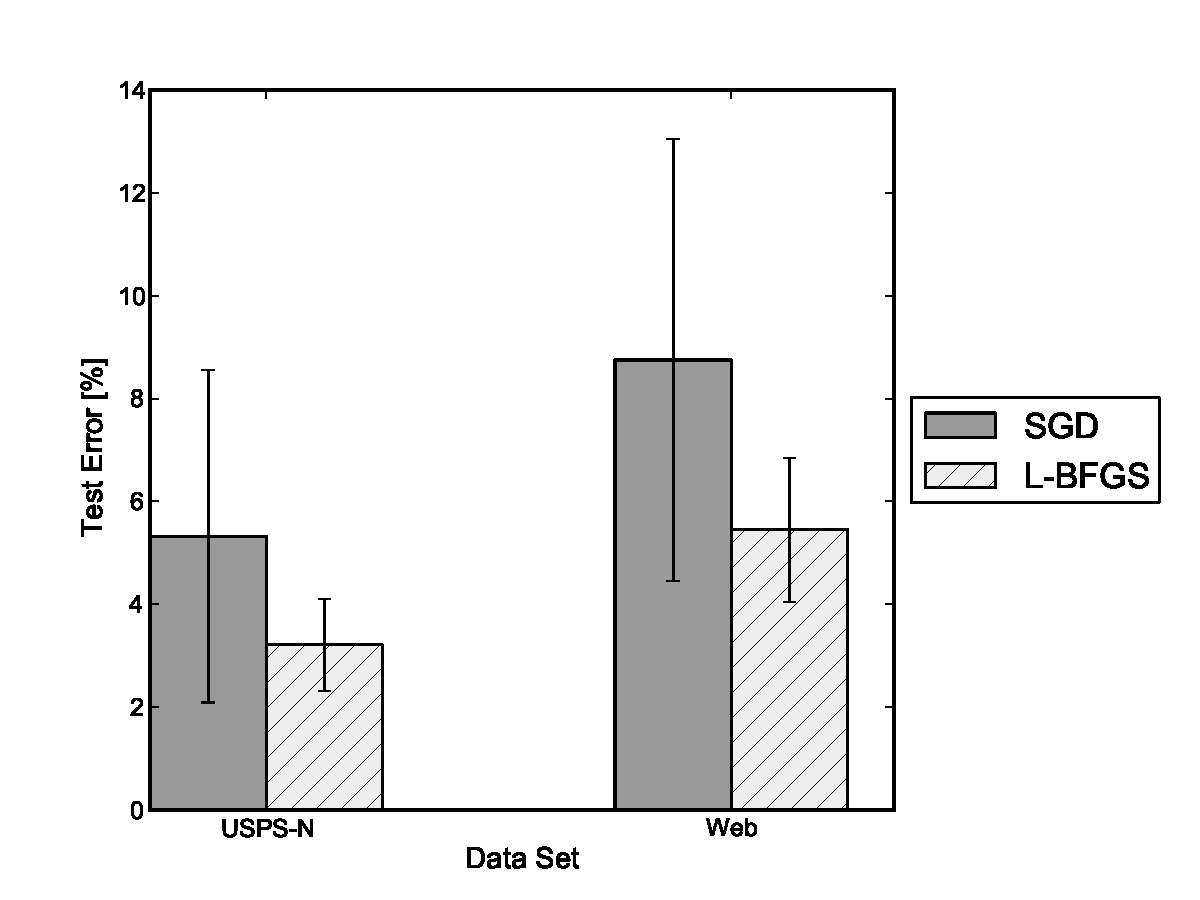
\includegraphics[width=1.0\textwidth]{test_error.pdf}
    \caption{Comparison of SGD and L-BFGS for USPS-N (left) and Web (right) data sets.}
\end{center}
\end{figure}


%-----------------------------------------------------------------------------
% FINDINGS AND LESSONS LEARNED
%-----------------------------------------------------------------------------
\section{Findings and Lessons Learned}
\label{sec:conclusion}

Findings and lessons learned.



%-----------------------------------------------------------------------------
% BIBLIOGRAPHY
%-----------------------------------------------------------------------------
\bibliographystyle{IEEEtran}
\bibliography{sources}


\end{document}
